\subsection{Class Diagrams}


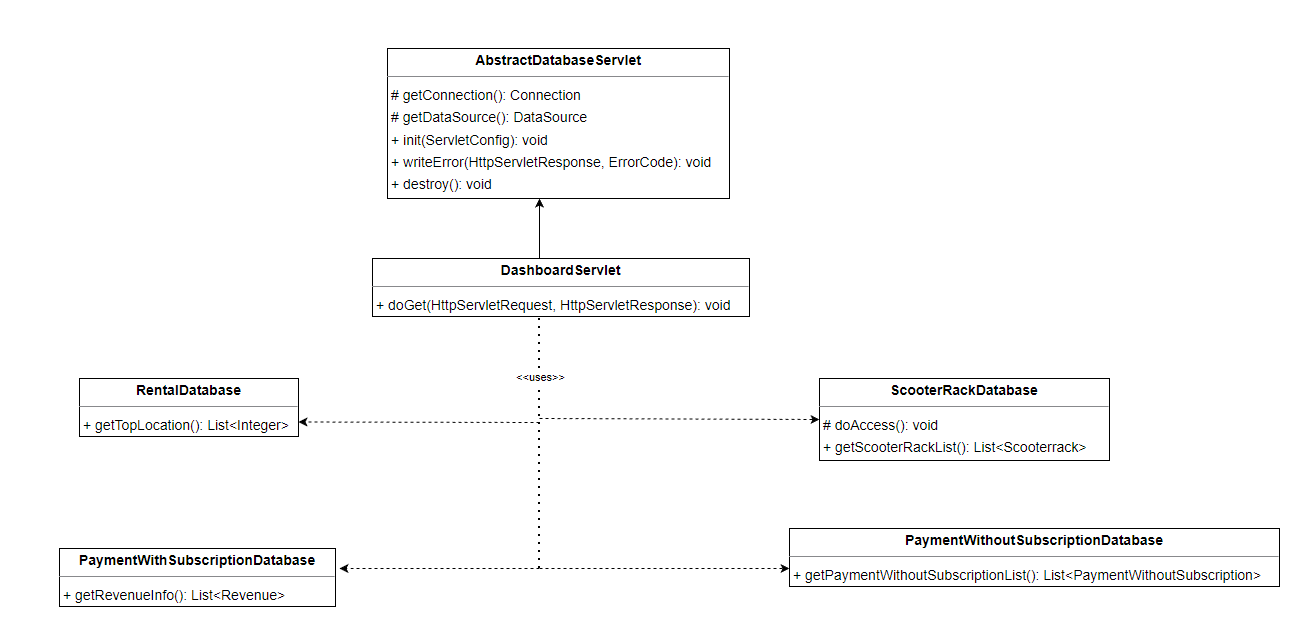
\includegraphics[scale=0.5]{sections/DLL/dashboard-servlet_CD.png}
This servlet uses the classes shown to access the database. This class diagram represents the classes involved in the dashboard servlet, which manages the dashboard page, it contains (some of) the classes used to handle three types of resources:scooter-Rack-List, top location, and revenue info. We used the proper queries to retrieve the necessary lists for each of these needed sections. For this, we used JDBC to establish a connection to the PostgreSQL database and ran the necessary queries from there. The desired tables were extracted, and the extracted queries were then turned into Java objects, and we used the proper queries to return the necessary lists for each of these desired sections. To achieve this, we used JDBC to establish a connection to the PostgreSQL database and ran the necessary queries. To present the collected data to the user, we had to extract from the relevant tables, turn the extracted queries into Java objects, and use JSP and HttpServlet technologies. 

As a result, we developed a servlet called dashboard servlet, and called the resources we already had, turned them into the appropriate Java models, then sent the desired characteristics to the page using the HttpServlet's APIs. We transferred the Jsp there and showed it, along with the following descriptions of the aforementioned sections.

\begin{enumerate}
    \item \textbf{scooterRackList}: shows a list of all locations where scooter rentals are available.
    \item \textbf{revenueInfo}: this shows the overall amount of money we made from renting scooters and our monthly income from scooter rentals.
    \item \textbf{top location}: using this reasoning, we can identify the city's busiest scooter rental location.
\end{enumerate}

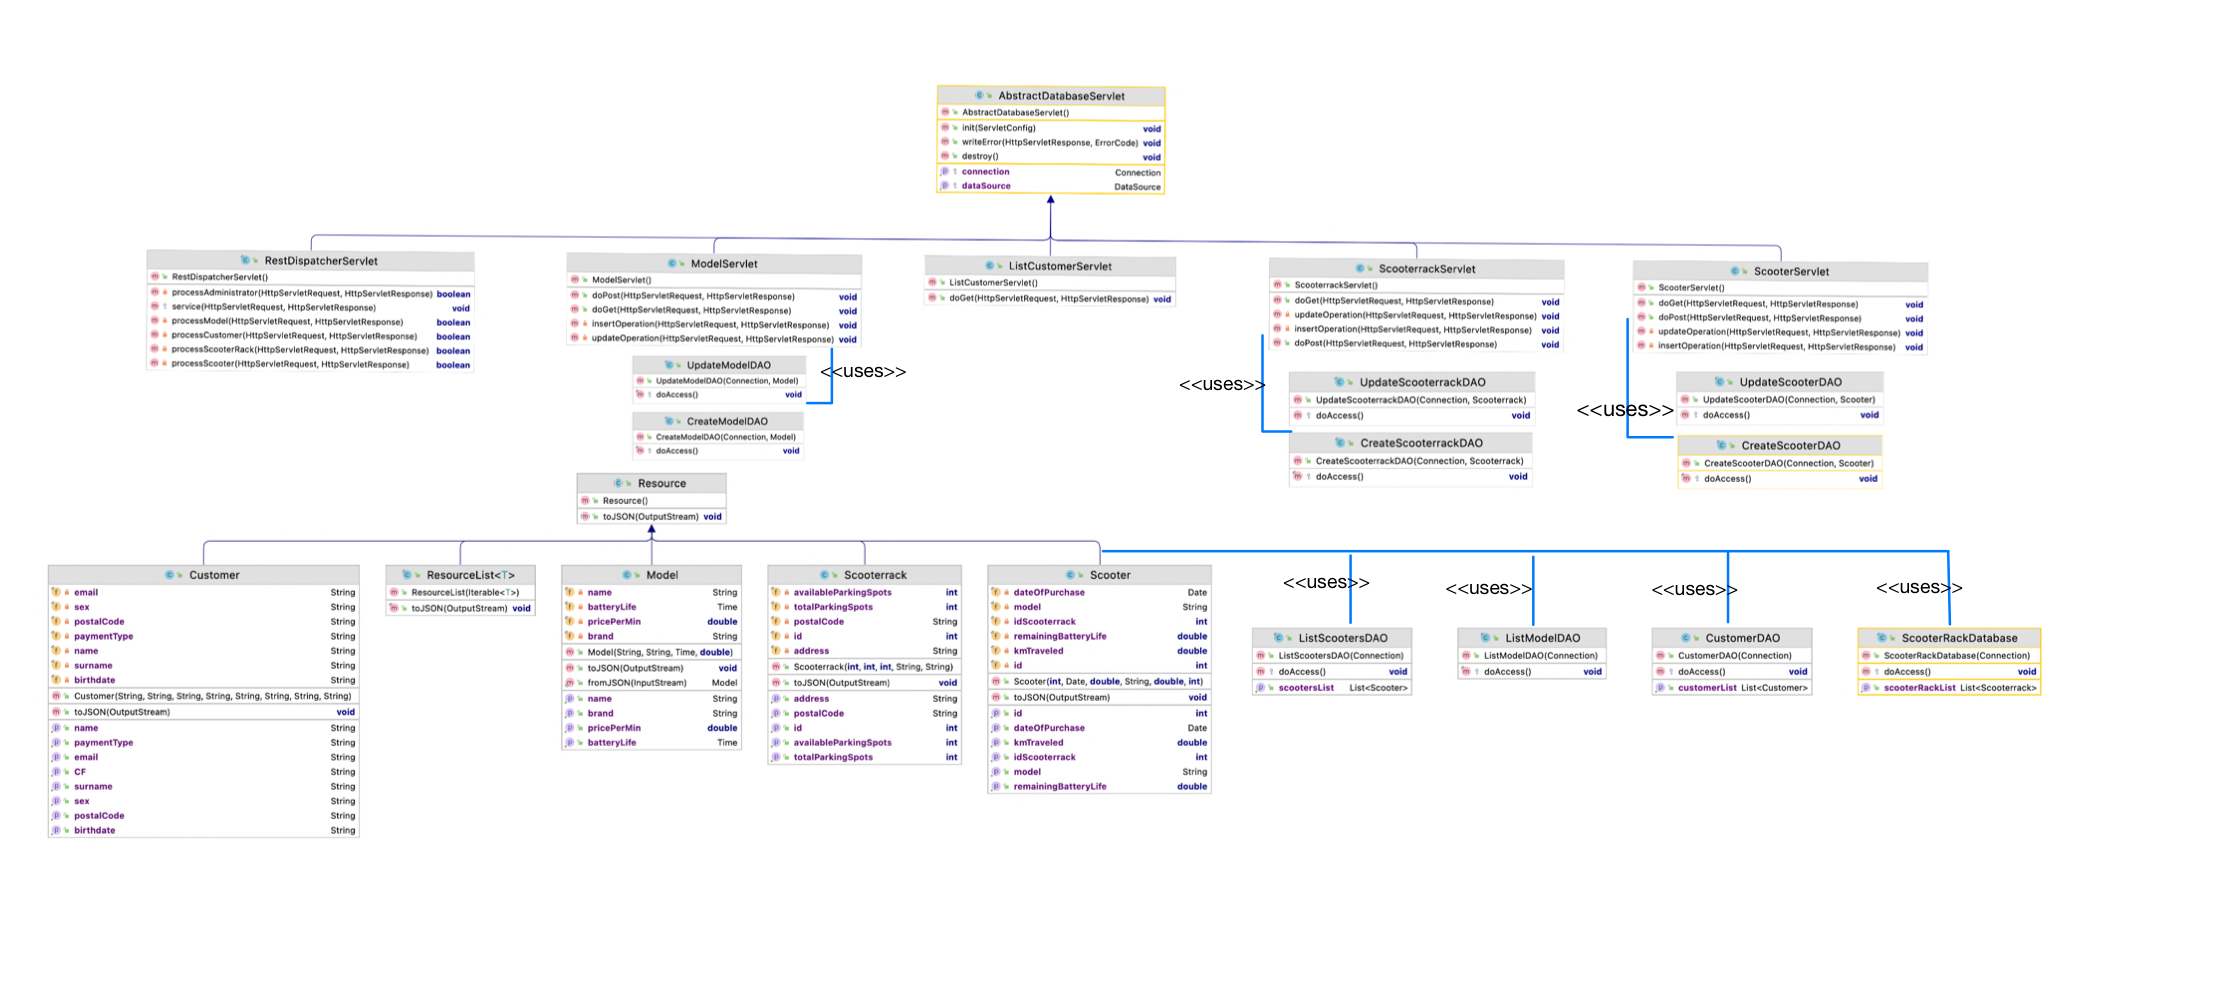
\includegraphics[scale=0.25]{sections/DLL/manage-servlet-rest.jpeg}

The second diagram represent the manage pages servlet and rest. The manage pages are model, scooter, scooter rack, rental, payment methods, customer and subscription. On these pages, we can interact with the respective tables of the database, for example: to view the list and add or edit that entity. In this case, we show the scooter, scooterracks, model and customer entities and have a servlet for viewing the list of scooters, one for adding a new scooter and one for editing an existing scooter. Then we also provide the REST API for getting the list of these entites. Both the rest and the servlets use some classes to access the database, as shown in the diagram. 